\section{Case Study 1: Spatial SIR} %(First Encounter)
\label{sec:cs_sir}

Our first case study is the SIR model which is a very well studied and understood compartment model from epidemiology \cite{kermack_contribution_1927} which allows to simulate the dynamics of an infectious disease like influenza, tuberculosis, chicken pox, rubella and measles spreading through a population \cite{enns_its_2010}.

In it, people in a population of size $N$ can be in either one of three states \textit{Susceptible}, \textit{Infected} or \textit{Recovered} at a particular time, where it is assumed that initially there is at least one infected person in the population. People interact \textit{on average} with a given rate of $\beta$ other people per time-unit and become infected with a given probability $\gamma$ when interacting with an infected person. When infected, a person recovers \textit{on average} after $\delta$ time-units and is then immune to further infections. An interaction between infected persons does not lead to re-infection, thus these interactions are ignored in this model. 

We followed in our agent-based implementation of the SIR model the work \cite{macal_agent-based_2010} but extended it by placing the agents on a discrete 2D grid using a Moore (8) neighbourhood TODO: cite my own PFE paper. In this case agents interact with each other indirectly through the shared discrete 2D grid by writing their current state on their cell which neighbours can read. A visualisation can be seen in Figure \ref{fig:vis_sir}.

It is important to note that due to the continuous-time nature of the SIR model, our implementation follows the time-driven \cite{meyer_event-driven_2014} approach and maps naturally to the continuous time-semantics and state-transitions provided by FRP. By sampling the system with very small $\Delta t$ this means that we have comparatively very few writes to the shared environment which will become important when discussing the performance results.

\begin{figure}
\begin{center}
	\begin{tabular}{c c}
		\begin{subfigure}[b]{0.4\textwidth}
			\centering
			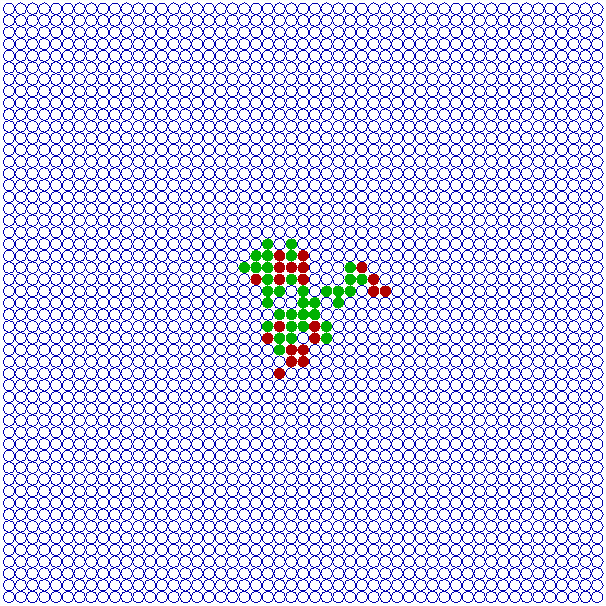
\includegraphics[width=1\textwidth, angle=0]{./fig/sir/vis/51x51agents_t50_01dt.png}
			\caption{$t = 50$}
			\label{fig:vis_51x51agents_t50_01dt}
		\end{subfigure}
    	
    	&
  
		\begin{subfigure}[b]{0.4\textwidth}
			\centering
			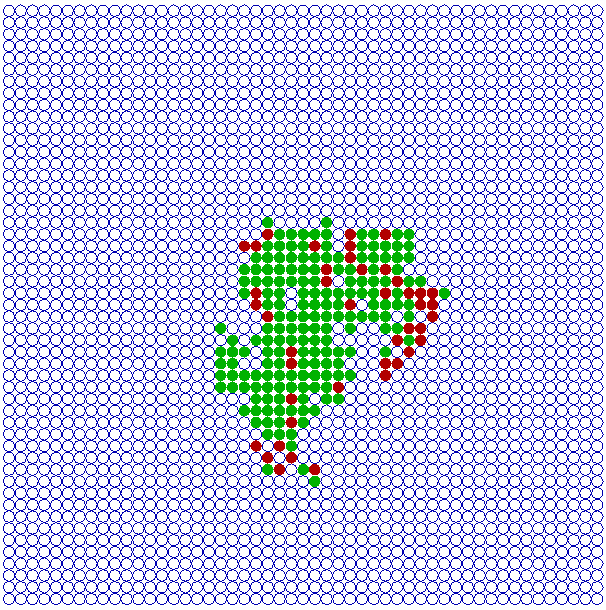
\includegraphics[width=1\textwidth, angle=0]{./fig/sir/vis/51x51agents_t100_01dt.png}
			\caption{$t = 100$}
			\label{fig:vis_51x51agents_t100_01dt}
		\end{subfigure}
	\end{tabular}
	
	\caption{Simulating the agent-based SIR model on a 51x51 2D grid with Moore neighbourhood, a single infected agent at the center, contact rate $\beta = \frac{1}{5}$, infection probability $\gamma = 0.05$ and illness duration $\delta = 15$ . Simulation run until $t = 100$ with fixed $\Delta t = 0.1$. The susceptible agents are rendered as blue hollow circles for better contrast.}
	\label{fig:vis_sir}
\end{center}
\end{figure}

\subsection{Experiment Design}
In this case study we compare the performance of the following implementations under varying numbers of CPU cores and agent numbers:

\begin{enumerate}
	\item Sequential - This is the original implementation we also discuss in TODO: cite my own PFE paper. In it the discrete 2D grid is shared amongst all agents using the State Monad. Agents are run sequentially after another thus ensuring exclusive read/write access to it. Because we are neither running in the STM or IO Monad there is no way we can run this implementation concurrently.
	\item STM - This is the same implementation like the State Monad but instead of sharing the discrete 2D grid in a State Monad, agents run in the STM Monad and have access to the discrete 2D grid through a transactional variable \textit{TVar}. This means that the reads and writes of the discrete 2D grid are exactly the same but happen always through the \textit{TVar}. Also each agent is run within its own thread, thus enabling true concurrency when the simulation is actually run on multiple cores (which can be configured by the Haskell Runtime System).
	\item Lock-Based - This is exactly the same implementation like the STM Monad but instead of running in STM, the agents now run in IO. They share the discrete 2D grid using an \textit{IORef} and have access to an \textit{MVar} to synchronise access to the it. Also each agent is run within its own thread.
	\item RePast - To have an idea where the functional implementation is performance-wise compared to the established object-oriented methods, we implemented a Java version of the SIR model using RePast with the State-Chart feature. This implementation cannot run on multiple cores concurrently but gives a good estimate of the single core performance of imperative approaches. Also there exists a RePast High Performance Computing library for implementing large-scale distributed simulations in C++ - we leave this for further research as an implementation and comparison is out of scope of this paper.
\end{enumerate}

Each experiment was run until $t = 100$ and stepped using $\Delta t = 0.1$ except in RePast for which we don't have access to the underlying implementation of the state-chart and left it as it is. For each experiment we conducted 8 runs on our machine (see Table \ref{tab:machine_specs}) under no additional work-load and report the average. Further, we checked the visual outputs and the dynamics and they look qualitatively the same to the reference implementation of the State Monad TODO: cite my own PFE paper. In the experiments we varied the number of agents (grid size) and the number of cores when running concurrently - the numbers are always indicated clearly. For varying the number of cores we compiled the executable using \textit{stack} and the \textit{threaded} option and executed it with \textit{stack} using the +RTS -Nx option where x is the number of cores between 1 and 4. 

\begin{table}
	\centering
	\begin{tabular}{ c || c }
		OS & Fedora 28 64-bit \\ \hline
		RAM & 16 GByte \\ \hline
		CPU & Intel Core i5-4670K @ 3.40GHz x 4 \\ \hline
		HD & 250Gbyte SSD \\ \hline
		Haskell & GHC 8.2.2 \\ \hline
		Java & OpenJDK 1.8.0 \\ \hline
		RePast & 2.5.0.a
	\end{tabular}
	
	\caption{Machine and Software Specs for all experiments}
	\label{tab:machine_specs}
\end{table}

\subsection{Constant Grid Size, Varying Cores}
In this experiment we held the grid size constant to 51 x 51 (2,601 agents) and varied the cores where possible. The results are reported in Table \ref{tab:constgrid_varyingcores}.

\begin{table}
	\centering
  	\begin{tabular}{ c || c | c  }
                    & Cores & Duration  \\ \hline \hline 
    	Sequential  & 1     & 100.3     \\ \hline \hline
   		STM         & 1     & 53.2      \\ \hline
   		STM         & 2     & 27.8      \\ \hline
   		STM         & 3     & 21.8      \\ \hline
   		STM         & 4     & 20.2      \\ \hline \hline
   		Lock-Based  & 1     & 60.6      \\ \hline 
   		Lock-Based  & 2     & 42.8      \\ \hline 
   		Lock-Based  & 3     & 38.6      \\ \hline 
   		Lock-Based  & 4     & 41.6      \\ \hline \hline
   		RePast      & 1     & \textbf{10.822} \\ \hline \hline
  	\end{tabular}
  	
  	\caption{Experiments on constant 51x51 (2,601 agents) grid with varying number of cores.}
	\label{tab:constgrid_varyingcores}
\end{table}

Comparing the performance and scaling on multiple cores of the STM and Lock-Based implementations shows that the lock-free STM implementation significantly outperforms the Lock-Based one and scales better to multiple cores. The Lock-Based implementation performs best with 3 cores and shows slightly worse performance on 4 cores as can be seen in Figure \ref{fig:core_duration_stm_io}. This is no surprise because the more cores are running at the same time, the more contention for the lock, thus the more likely synchronisation happening, resulting in more potential for reduced performance. This is not an issue in STM because no locks are taken in advance. 

Comparing the reference \textit{State} implementation shows that it is the slowest by far - even the single core STM and Lock-Based implementations outperform it by far. Also our profiling results reported about 30\% increased memory footprint for the State implementation. This shows that the State Monad is a rather slow and memory intense approach sharing data but guarantees purity and excludes any non-deterministic side-effects which is not the case in STM and IO.

What comes a bit as a surprise is that the single core RePast implementation significantly outperforms \textit{all} other implementations, even when they run on multiple cores and even with RePast doing complex visualisation in addition (something the functional implementations don't do). We attribute this to the conceptually slower approach of functional programming. We might could have optimised parts of the code but leave this for further research.

\begin{figure}
	\centering
	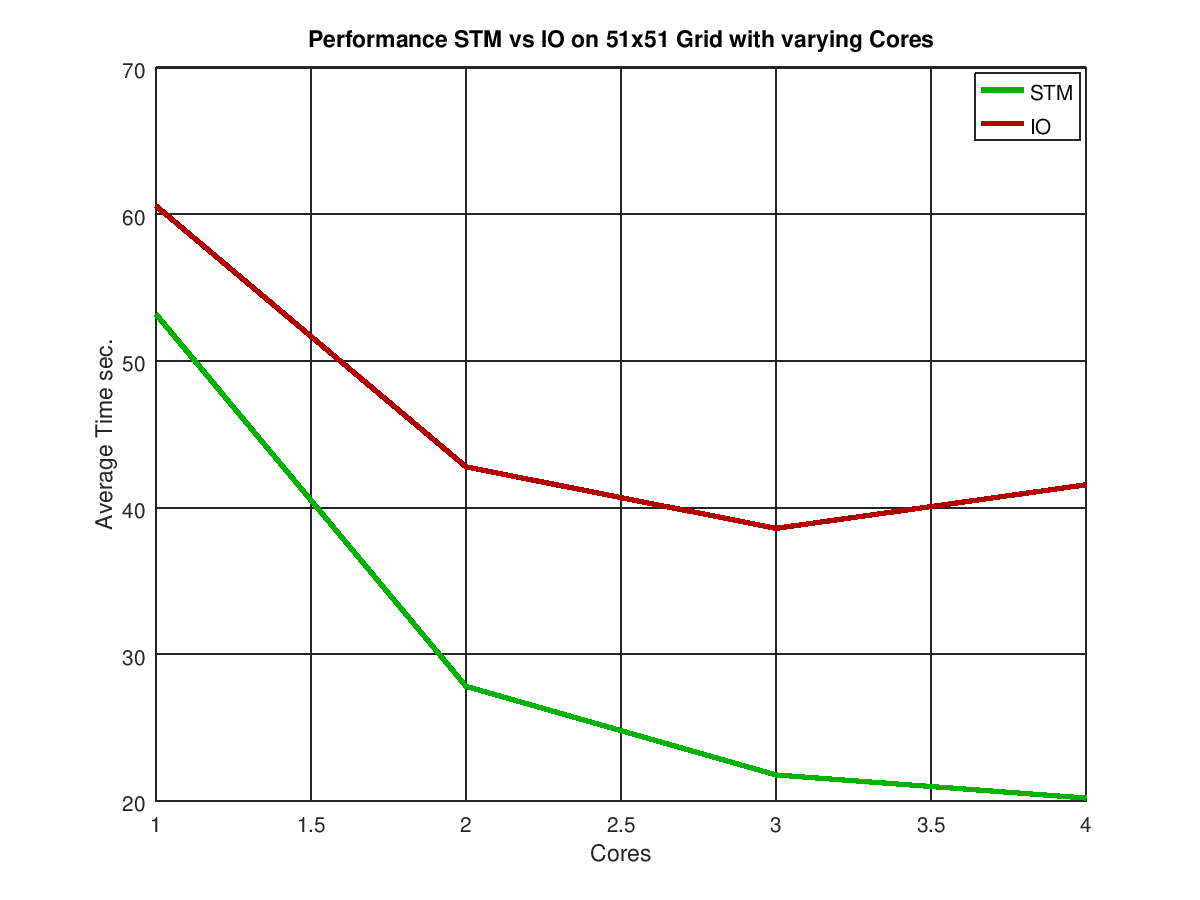
\includegraphics[width=0.6\textwidth, angle=0]{./fig/sir/core_duration_stm_io.png}
	\caption{Comparison of performance and scaling on multiple cores of STM vs. IO. Note that the Lock-Based implementation performs worse on 4 cores than on 3.}
	\label{fig:core_duration_stm_io}
\end{figure}

\subsection{Varying Grid Size, Constant Cores}
In this experiment we varied the grid size and used constantly 4 cores. Because in the previous experiment, Lock-Based performed best on 3 cores, we additionally ran Lock-Based on 3 cores as well. The results for STM are reported in Table \ref{tab:varyinggrid_constcores}. Again, note that the RePast experiments all ran on a single (1) core and were conducted to have a rough estimate where the functional approach is in comparison to the imperative.

\begin{table}
	\centering
  	\begin{tabular}{ c || c | c | c | c }
        Grid-Size          & STM              & Lock-Based (4 cores) & Lock-Based (3 cores) & RePast (1 core) \\ \hline \hline 
   		51 x 51 (2,601)    & 20.2             & 41.9                 & 38.6                 & \textbf{10.8}   \\ \hline
   		101 x 101 (1,0201) & \textbf{74.5}    & 170.5                & 171.6                & 107.40          \\ \hline
   		151 x 151 (22,801) & \textbf{168.5}   & 376.9                & 404.1                & 464.017         \\ \hline
   		201 x 201 (40,401) & \textbf{302.4}   & 672.0                & 720.6                & 1,227.68        \\ \hline
   		251 x 251 (63,001) & \textbf{495.7}   & 1,027.3              & 1,117.2              & 3,283.63        \\ \hline \hline
  	\end{tabular}

  	\caption{Performance on varying grid sizes.}
	\label{tab:varyinggrid_constcores}
\end{table}

We plotted the results in Figure \ref{fig:stm_io_repast_varyinggrid_performance}. It is clear that the lock-free STM implementation outperforms the lock-based Lock-Based implementation by a substantial factor. Surprisingly, the Lock-Based implementation on 4 core scales just slightly better with increasing agents number than on 3 cores, something we wouldn't have anticipated based on the results seen in Table \ref{tab:constgrid_varyingcores}. Also  while on a 51x51 grid the single (1) core Java RePast version outperforms the 4 core Haskell STM version by a factor of 2. The figure is inverted on a 251x251 grid where the 4 core Haskell STM version outperforms the single core Java Repast version by a factor of 6. This might not be entirely surprising because we compare single (1) core against multi-core performance - still the scaling is indeed impressive and we would never have anticipated an increase of factor 6.

\begin{figure}
\begin{center}
	\begin{tabular}{c c}
		\begin{subfigure}[b]{0.5\textwidth}
			\centering
			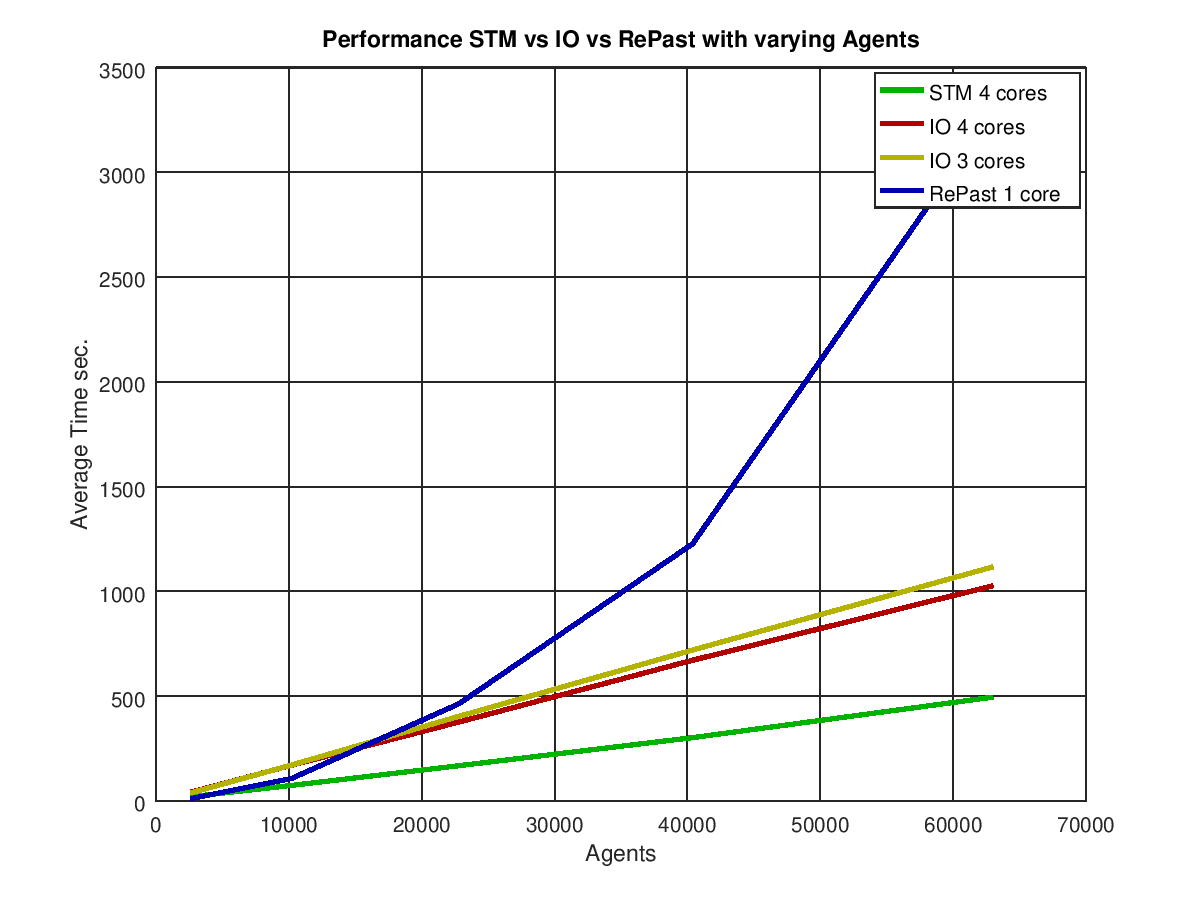
\includegraphics[width=1\textwidth, angle=0]{./fig/sir/stm_io_repast_varyinggrid_performance.png}
			\caption{Normal Scale}
		\end{subfigure}
    	&
		\begin{subfigure}[b]{0.5\textwidth}
			\centering
			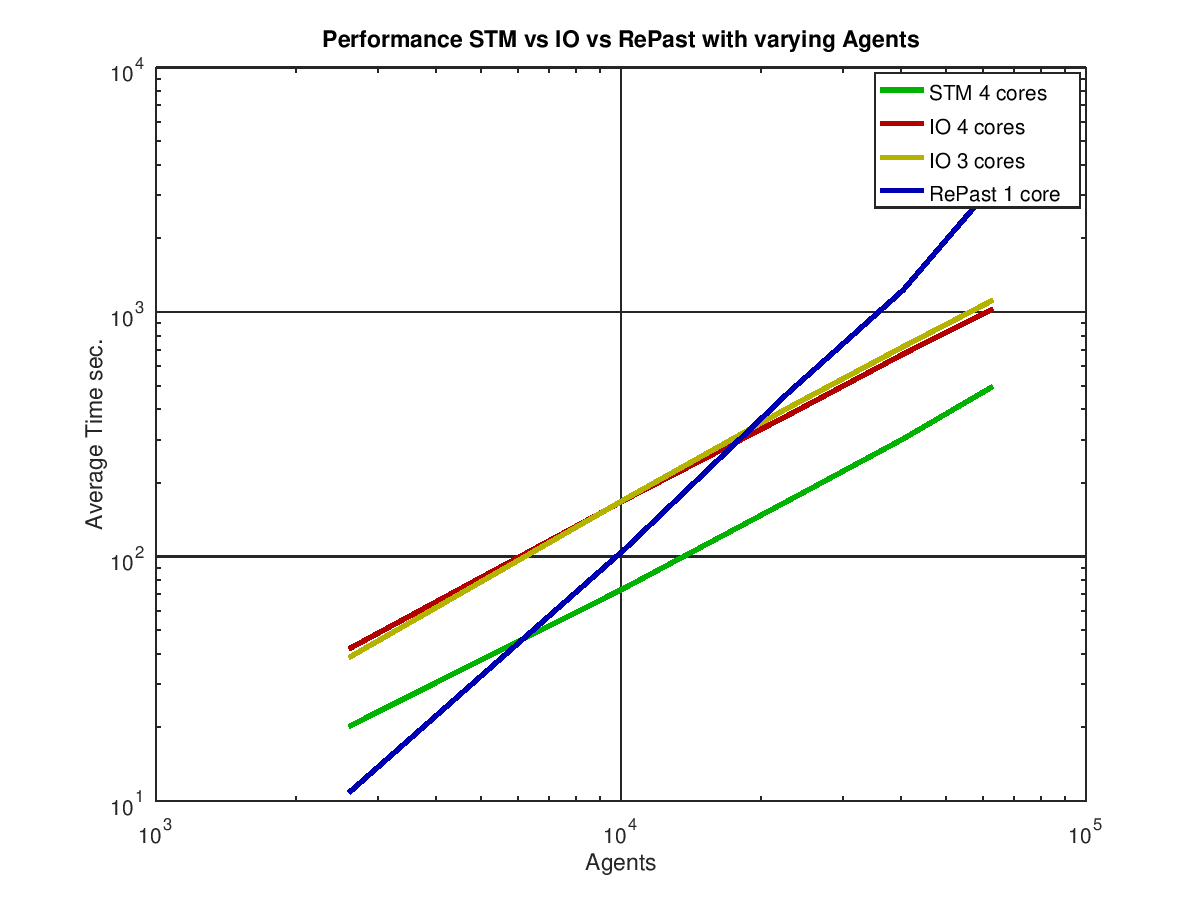
\includegraphics[width=1\textwidth, angle=0]{./fig/sir/stm_io_repast_varyinggrid_performance_loglog.png}
			\caption{Logarithmic scale on both axes}
		\end{subfigure}
    \end{tabular}
	\caption{Performance on varying grid sizes.}
	\label{fig:stm_io_repast_varyinggrid_performance}
\end{center}
\end{figure}

\subsection{Retries}
Of very much interest when using STM is the retry-ratio, which obviously depends highly on the read-write patterns of the respective model. We used the stm-stats library to record statistics of commits, retries and the ratio. In these experiments we only averaged over 4 runs because they all arrived at a ratio of 0.0. The results are reported in Table \ref{tab:retries_stm}.

\begin{table}
	\centering
  	\begin{tabular}{ c || c | c | c }
        Grid-Size 		   & Commits    & Retries & Ratio \\ \hline \hline 
   		51 x 51 (2,601)    & 2,601,000  & 1306.5  & 0.0 \\ \hline
   		101 x 101 (10,201) & 10,201,000 & 3712.5  & 0.0 \\ \hline
   		151 x 151 (22,801) & 22,801,000 & 8189.5  & 0.0 \\ \hline
   		201 x 201 (40,401) & 40,401,000 & 13285   & 0.0 \\ \hline 
   		251 x 251 (63,001) & 63,001,000 & 21217   & 0.0 \\ \hline \hline
  	\end{tabular}
  	
  	\caption{Retries Ratio of STM Monad experiments on varying grid sizes on 4 cores.}
	\label{tab:retries_stm}
\end{table}

Independent of the number of agents we always have a retry-ratio of 0.0. This indicates that this model is \textit{very} well suited to STM, which is also directly reflected in the substantial better performance over the Lock-Based implementation. Obviously this ratio stems from the fact, that in our implementation we have \textit{very} few writes (only when an agent changes e.g. from Susceptible to Infected or from Infected to Recovered) and mostly reads. Also we conducted runs on lower number of cores which resulted in fewer retries, which was what we expected.

\subsection{Going Large-Scale}
To test how far we can scale up the number of cores in both the \textit{Lock-Based} and \textit{STM} cases, we ran the two experiments (51x51 and 251x251) on Amazon S2 instances with increasing number of cores starting with 16 until we ran into decreasing returns. The results are reported in Table \ref{tab:sir_varying_cores_amazon}.

\begin{table}
	\centering
  	\begin{tabular}{ c || c | c | c }
                   & Cores & 51x51   & 251x251 \\ \hline \hline 
    	Lock-Based & 16    & 72.5    & TODO    \\ \hline
    	Lock-Based & 32    & 73.1    & TODO    \\ \hline \hline 
   		
   		STM        & 16    & 8.6     & 237.0   \\ \hline
   		STM        & 32    & 12.0    & 248.7   \\ \hline \hline
   	\end{tabular}
  	
  	\caption{Performance on varying cores on Amazon S2 Services.}
	\label{tab:sir_varying_cores_amazon}
\end{table}

As expected, the \textit{Lock-Based} approach doesn't scale up to many cores because each additional core brings more contention to the lock, resulting in even more decreased performance. This is particularly obvious in the 251x251 experiment because of the much larger number of concurrent agents. The \textit{STM} approach returns better performance on 16 cores but fails to scale further up to 32 where the performance drops below the one with 16 cores. %At this point we are running into Amdahls law and become dominated by the sequential part of the program which is the main lock-step mechanism. 

TODO: why? need to check retries  
TODO: the INCREASE in time can only happen due to more retries 
16 cores 251x251: 0.0 retry-ratio
32 cores 251x251: 0.0 retry ratio

16 cores 51x51: 0.0 retry-ratio
32 cores 51x51: 0.0 retry ratio

\subsection{Discussion}
Reflecting of the performance data leads to the following insights:
\begin{enumerate}
	\item Running in STM and sharing state using a transactional variable is much more time- and memory-efficient than running in the State Monad but potentially sacrifices determinism: repeated runs might not lead to same dynamics despite same initial conditions.
	\item Running STM on multiple cores concurrently \textit{does} lead to a significant performance improvement \textit{for that model}.
	\item STM outperforms the Lock-Based implementation substantially and scales much better to multiple cores.
	\item STM on single (1) core is still about twice as slow than an object-oriented Java RePast implementation on a single (1) core.
	\item STM on multiple cores dramatically outperforms the single (1) core object-oriented Java RePast implementation on a single (1) core on instances with large agent numbers and scales much better to increasing number of agents.
\end{enumerate}